\documentclass[a4paper, 11pt]{article}
\usepackage{config}

\begin{document}

\thispagestyle{empty}
\tableofcontents

\newpage
\section{Metamodelos}

\begin{figure}[H]
\centering
\begin{minipage}{.4\textwidth}
  \centering
  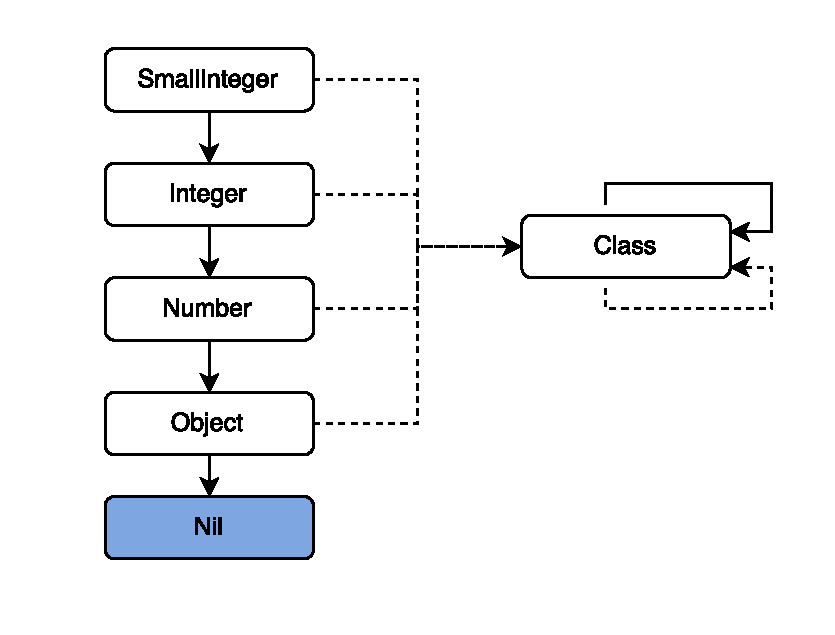
\includegraphics[width=\linewidth]{images/metamodelo_smalltalk_basico.pdf}
  \caption{Metamodelo B\'asico}
  \label{fig:metamodelo_basico}
\end{minipage}%
\begin{minipage}{.6\textwidth}
  \centering
  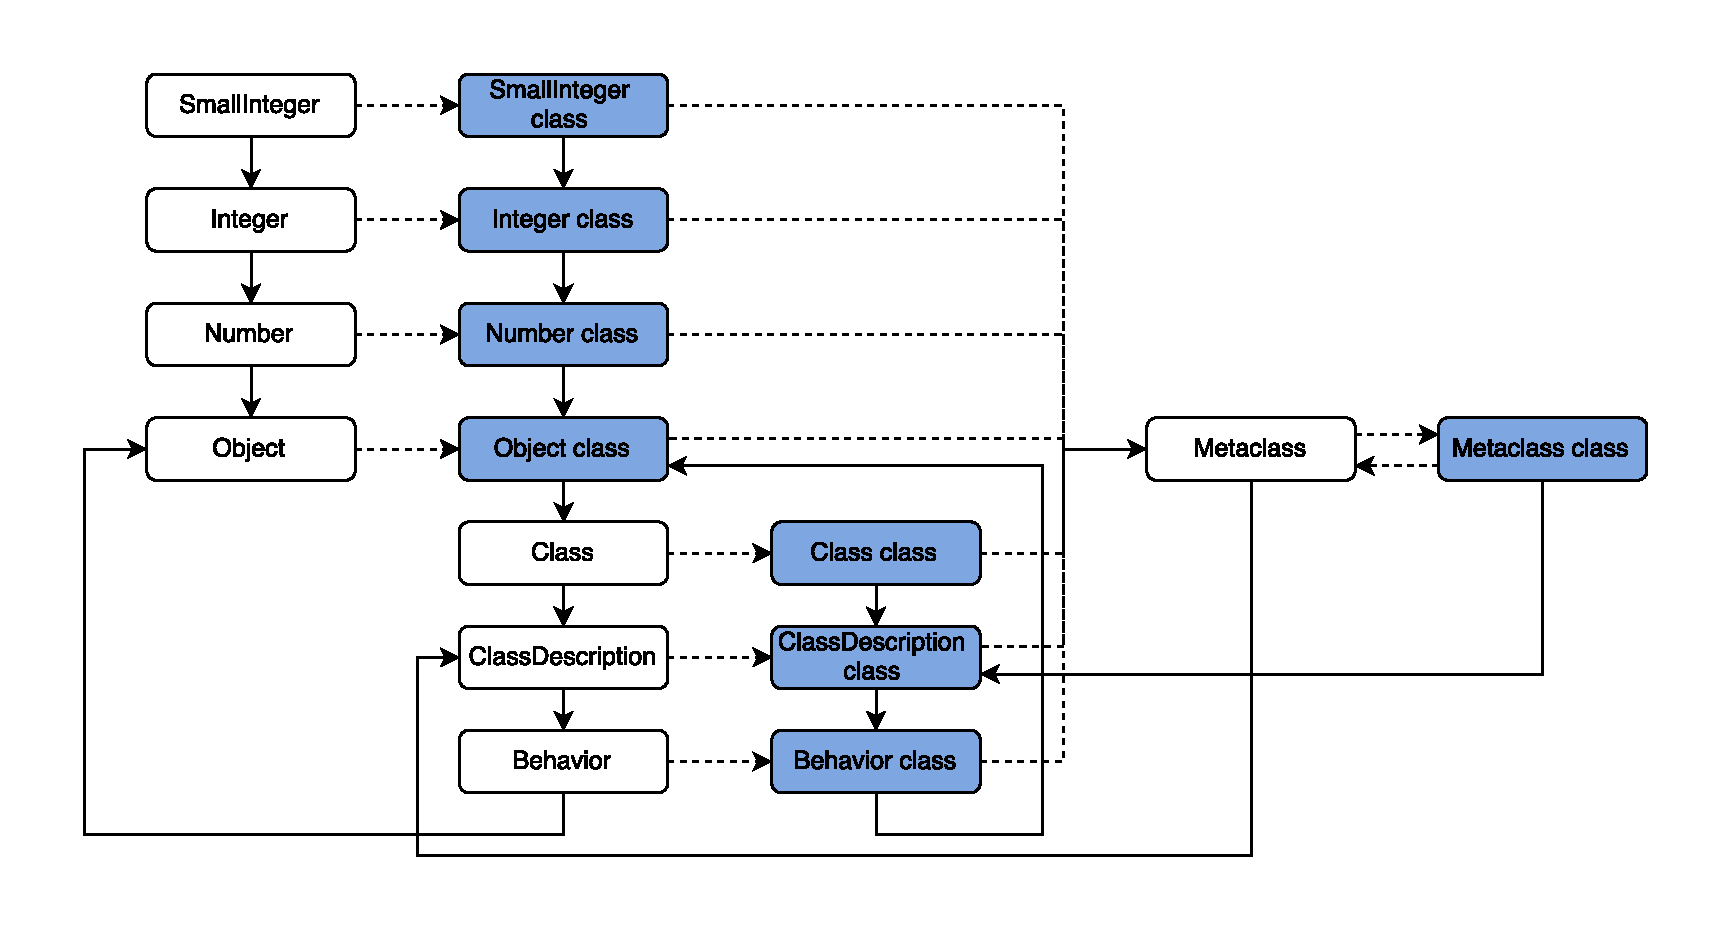
\includegraphics[width=1.2\linewidth]{images/metamodelo_smalltalk_80.pdf}
  \caption{Metamodelo SmallTalk80}
  \label{fig:metamodelo_st80}
\end{minipage}
\label{fig:test}
\end{figure}

\begin{figure}[H]
  \begin{center}
  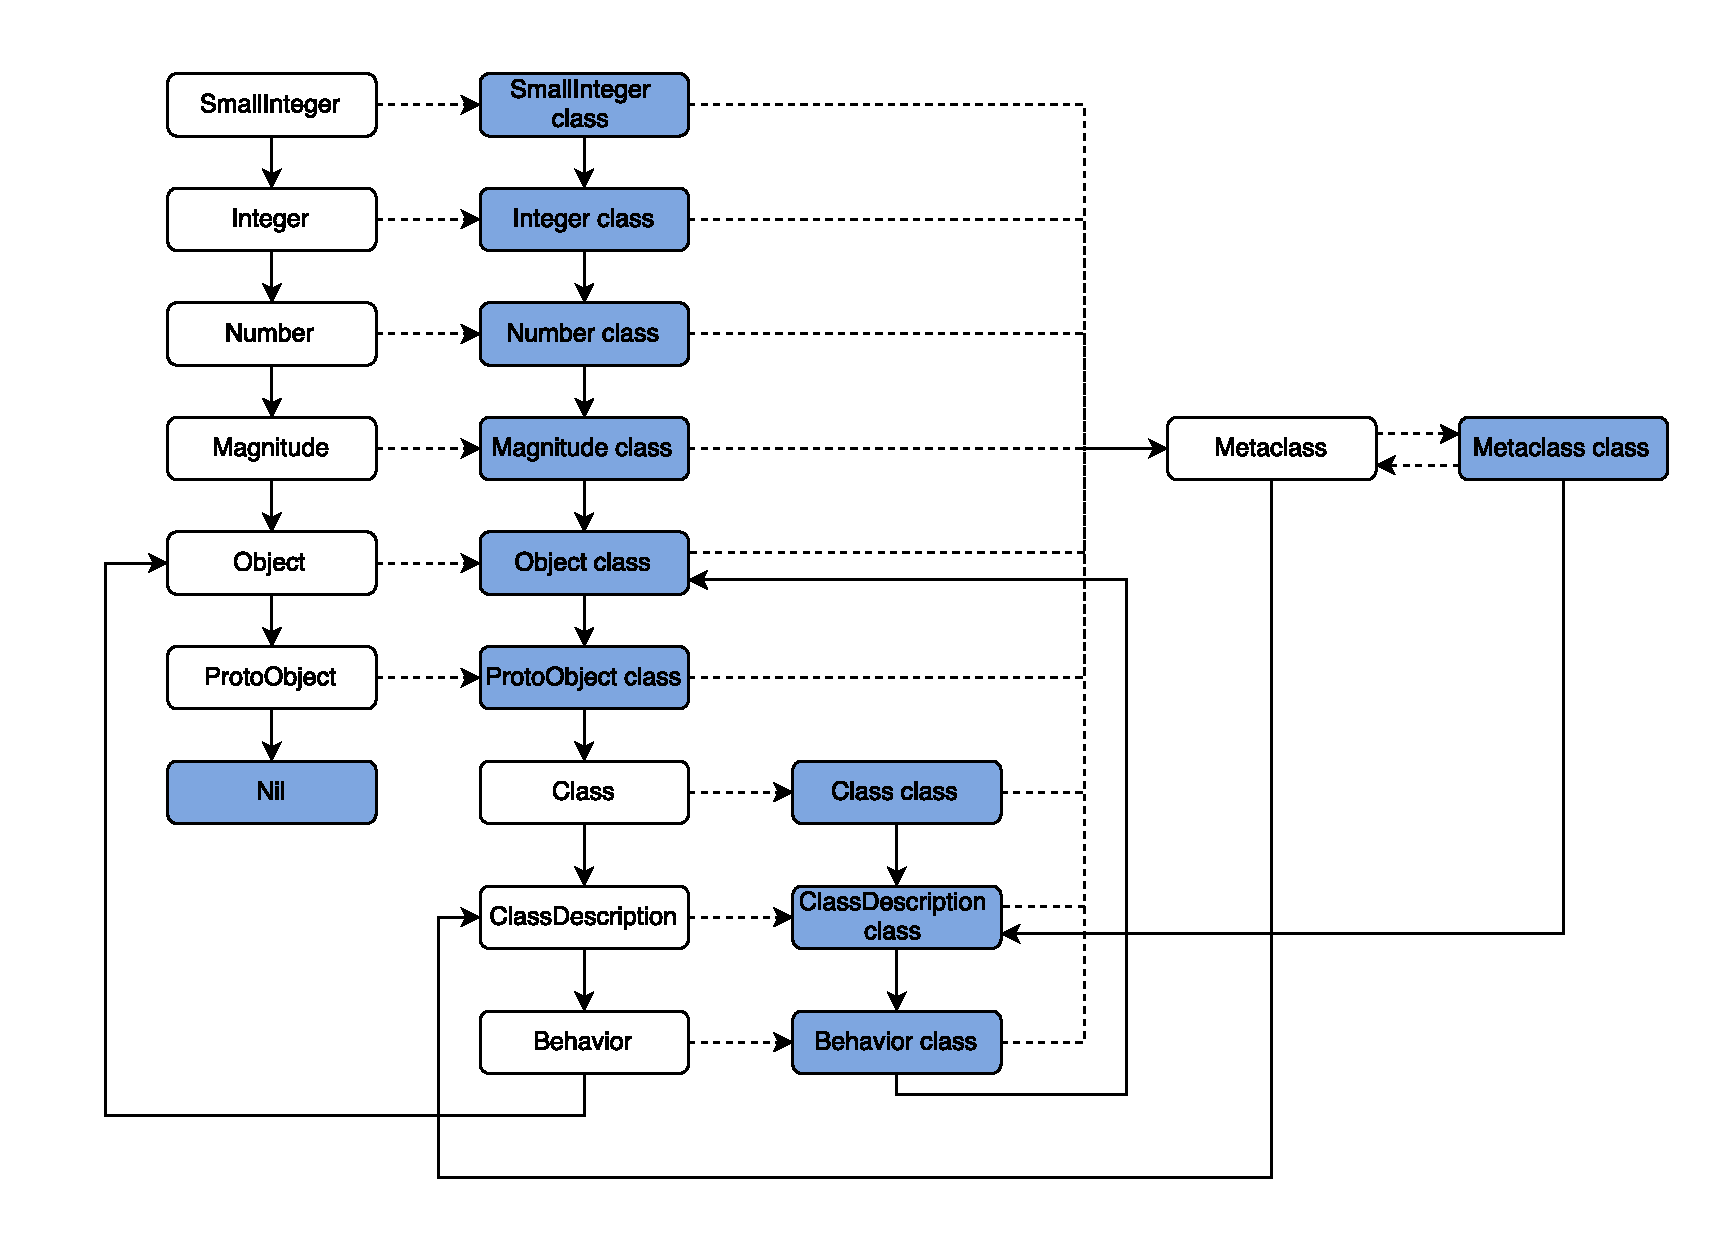
\includegraphics[height=300px]{images/metamodelo_smalltalk.pdf}
  \end{center}
  \caption{Metamodelo de Pharo4.0}
  \label{fig:metamodelo_pharo}
\end{figure}

\begin{figure}[H]
\centering
\begin{minipage}{.5\textwidth}
  \centering
  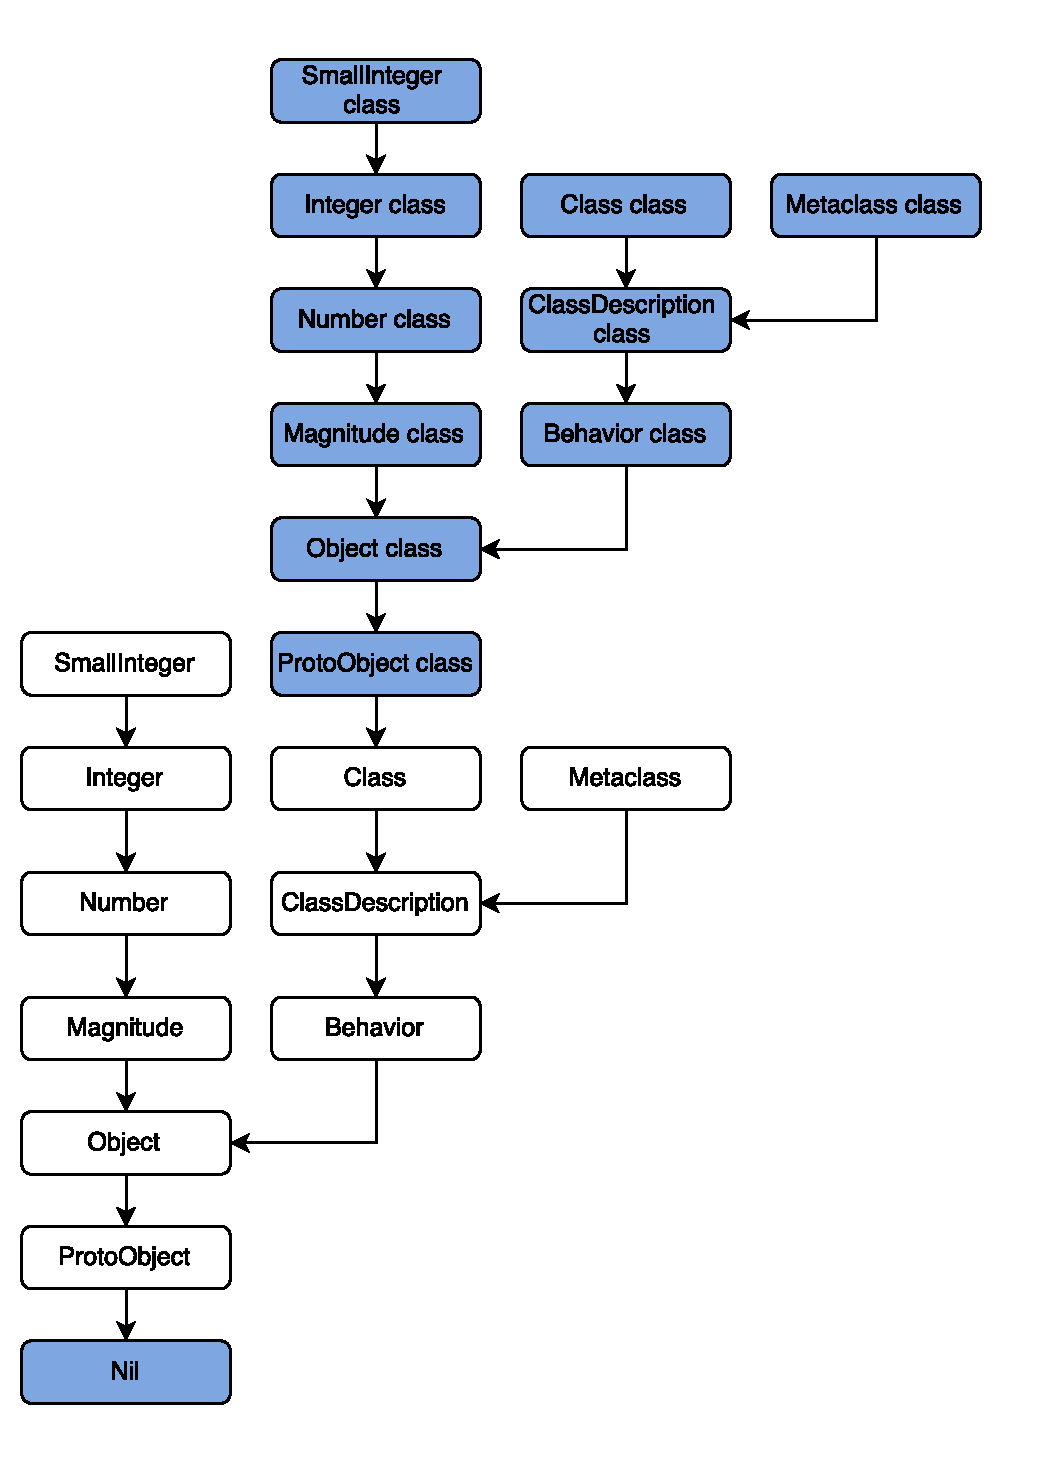
\includegraphics[width=\linewidth]{images/metamodelo_superclases.pdf}
  \caption{Grafo de Subclasificaciones}
  \label{fig:sub1}
\end{minipage}%
\begin{minipage}{.5\textwidth}
  \centering
  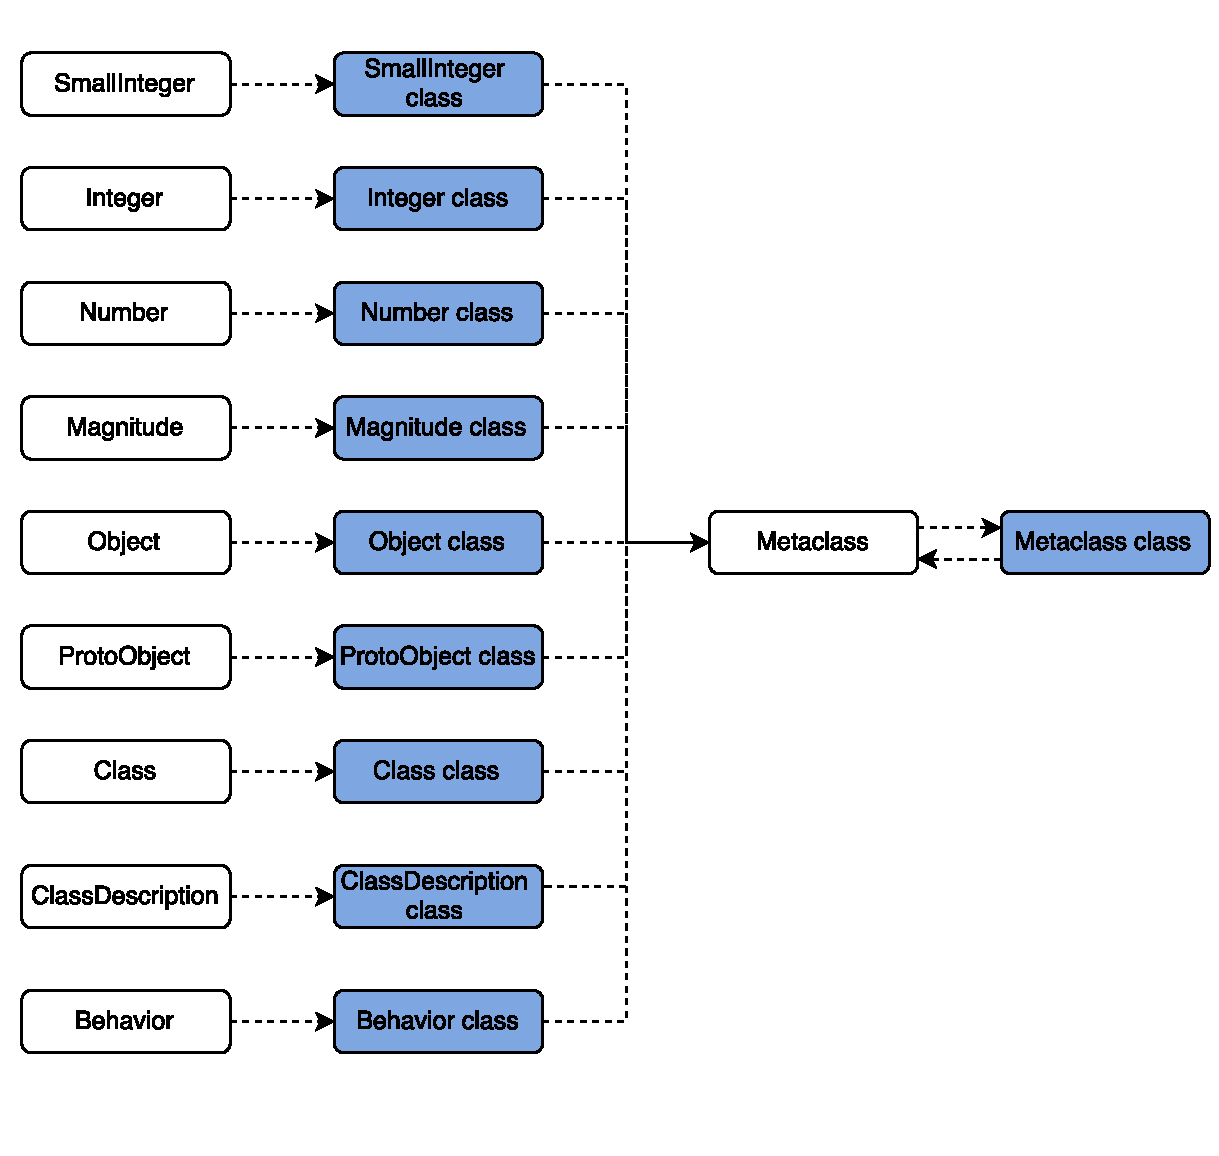
\includegraphics[width=1.2\linewidth]{images/metamodelo_instancia_de.pdf}
  \caption{Grafo ``Instancia de''}
  \label{fig:sub2}
\end{minipage}
\caption{Metamodelo de Pharo4.0}
\label{fig:test}
\end{figure}

\underline{Referencias}: Linea punteada significa ``Instancia de'', y Linea lisa ``Hereda de''.

\begin{enumerate}
 \item Los objetos en azul (?`las metaclases?), solo tienen una instancia. No contestan al mensaje \texttt{new}. ?`Qui\'en hace la alocaci\'on por primera vez? 
 
 Si a una metaclase se le agregan variables de instancia que inicializo en su m\'etodo \texttt{initialize} pero luego las modifico, debo reinicializar la metaclase para que se apliquen los cambios a las variables. No es como el caso de las variables de instancia de una clase. 
 
 \item Cuando se env\'ia \texttt{new} a cualquier objeto, el que aloca la memoria es \texttt{Behavior>>basicNew}. 
  \begin{enumerate}
    \item ?`Hace falta entonces dentro de cualquier implementaci\'on propia de \texttt{new} enviar la colaboraci\'on \texttt{super new} necesariamente??`Si no lo hago alguien se encarga de esto? 
    \item Si es \texttt{Behavior} quien implementa la alocaci\'on, ?`qui\'en lo hace para \texttt{Object} y los que subclasifican de \'el? (El debugger no me deja meterme m\'as adentro del \texttt{self new initialize} de \texttt{Object})
    
     \item \texttt{ProtoObject new} tira el siguiente error y se rompe todo: 

	\begin{verbatim}
	*** System error handling failed ***
	Original error: MessageNotUnderstood: ProtoObject>>inspect.
	\end{verbatim}

	?`Tiene algo que ver?
    
  \end{enumerate}

 \item Enviarle la colaboraci\'on \texttt{superclass} a un objeto me devuelve lo que apunta la flecha lisa. Ej: 
\begin{verbatim}
SmallInteger superclass
>> Integer
Metaclass superclass
>> ClassDescription
\end{verbatim}

 \item Enviarle la colaboraci\'on \texttt{class} a un objeto me devuelve lo que apunta la flecha punteada. Ej: 
\begin{verbatim}
SmallInteger class
>> Smallinteger class
Integer class class
>> Metaclass
\end{verbatim}
  
 \item Enviar la colaboraci\'on \texttt{Metaclass new new} hace colgar Pharo. ?`Por qu\'e? ?`Es el \'unico objeto con el que pasa eso? 

\end{enumerate}




\end{document}
